% Created by tikzDevice version 0.12.3.1 on 2021-05-03 23:03:23
% !TEX encoding = UTF-8 Unicode
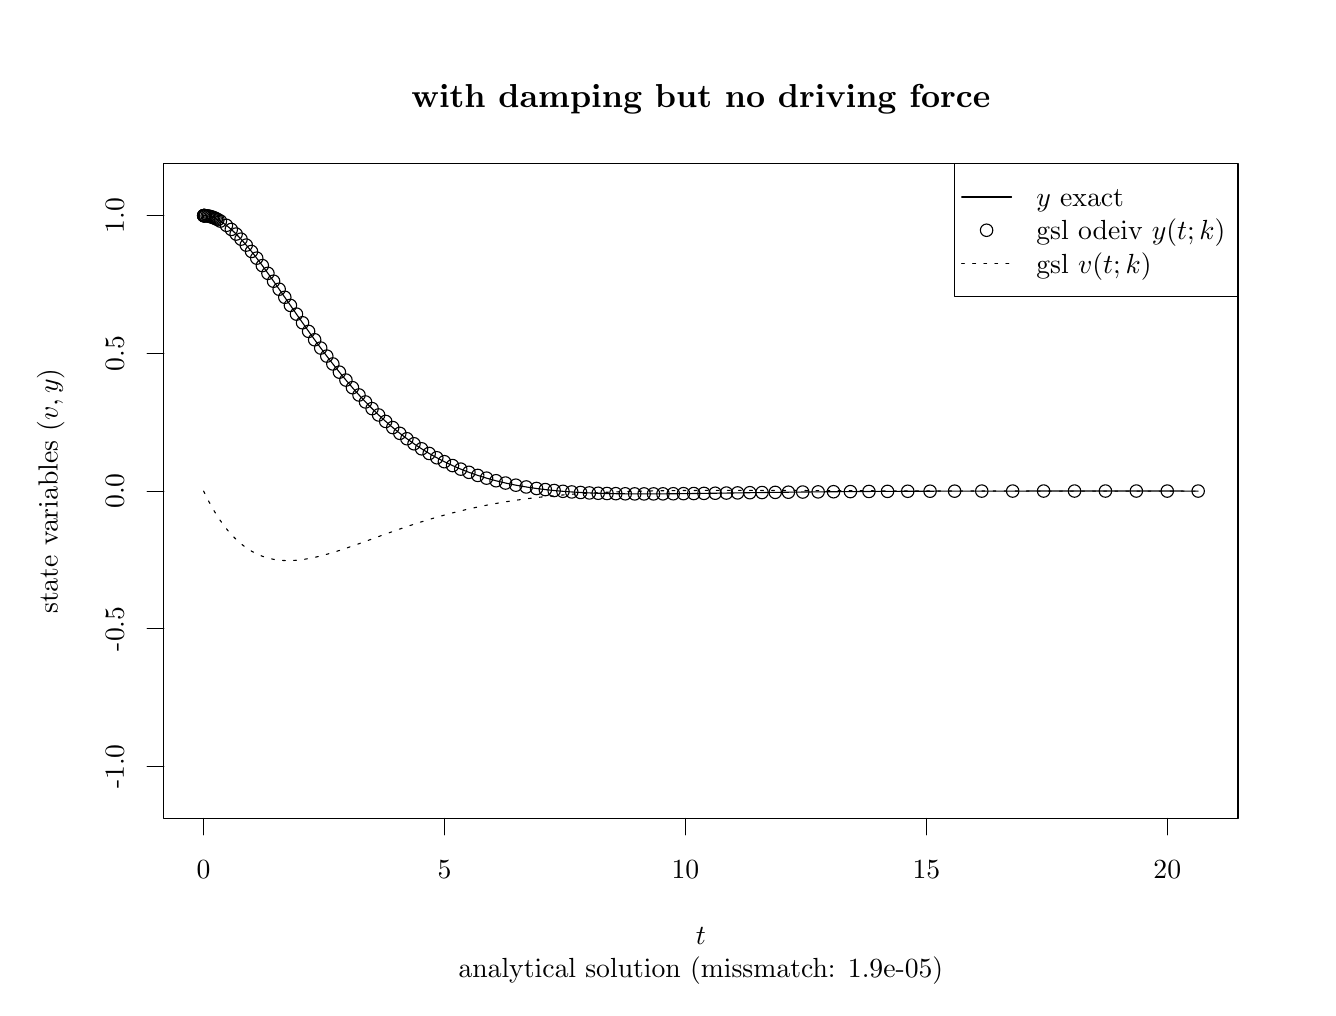
\begin{tikzpicture}[x=1pt,y=1pt]
\definecolor{fillColor}{RGB}{255,255,255}
\path[use as bounding box,fill=fillColor,fill opacity=0.00] (0,0) rectangle (462.53,346.90);
\begin{scope}
\path[clip] ( 49.20, 61.20) rectangle (437.33,297.70);
\definecolor{drawColor}{RGB}{0,0,0}

\path[draw=drawColor,line width= 0.4pt,line join=round,line cap=round] ( 63.58,278.98) --
	( 63.62,278.98) --
	( 63.66,278.98) --
	( 63.70,278.98) --
	( 63.74,278.98) --
	( 63.79,278.98) --
	( 63.88,278.98) --
	( 64.02,278.97) --
	( 64.28,278.95) --
	( 64.85,278.89) --
	( 65.32,278.81) --
	( 65.79,278.70) --
	( 66.27,278.57) --
	( 66.74,278.41) --
	( 67.21,278.24) --
	( 67.69,278.04) --
	( 68.16,277.82) --
	( 68.75,277.52) --
	( 69.64,277.00) --
	( 71.82,275.48) --
	( 73.58,274.00) --
	( 75.33,272.32) --
	( 77.09,270.48) --
	( 78.98,268.33) --
	( 80.88,266.03) --
	( 82.77,263.61) --
	( 84.80,260.92) --
	( 86.82,258.13) --
	( 88.85,255.28) --
	( 90.88,252.39) --
	( 92.91,249.47) --
	( 94.94,246.55) --
	( 97.13,243.39) --
	( 99.32,240.26) --
	(101.51,237.17) --
	(103.70,234.12) --
	(105.89,231.14) --
	(108.08,228.22) --
	(110.27,225.39) --
	(112.64,222.42) --
	(115.00,219.56) --
	(117.36,216.81) --
	(119.72,214.18) --
	(122.08,211.65) --
	(124.45,209.25) --
	(126.81,206.96) --
	(129.37,204.61) --
	(131.92,202.40) --
	(134.48,200.32) --
	(137.04,198.37) --
	(139.60,196.54) --
	(142.34,194.72) --
	(145.08,193.04) --
	(147.83,191.49) --
	(150.57,190.06) --
	(153.52,188.66) --
	(156.48,187.38) --
	(159.43,186.23) --
	(162.62,185.11) --
	(165.81,184.12) --
	(169.24,183.17) --
	(172.67,182.35) --
	(176.40,181.58) --
	(180.14,180.93) --
	(183.87,180.38) --
	(187.06,179.98) --
	(190.24,179.64) --
	(193.42,179.36) --
	(196.61,179.13) --
	(199.79,178.94) --
	(202.97,178.78) --
	(206.16,178.66) --
	(209.34,178.57) --
	(212.52,178.50) --
	(215.93,178.46) --
	(219.34,178.43) --
	(222.74,178.42) --
	(226.15,178.43) --
	(229.56,178.45) --
	(233.27,178.48) --
	(236.97,178.52) --
	(240.68,178.56) --
	(244.38,178.61) --
	(248.43,178.67) --
	(252.48,178.73) --
	(256.53,178.79) --
	(260.95,178.86) --
	(265.36,178.92) --
	(270.13,178.98) --
	(274.89,179.04) --
	(280.06,179.10) --
	(285.63,179.16) --
	(291.19,179.21) --
	(297.29,179.26) --
	(303.99,179.31) --
	(310.70,179.34) --
	(318.01,179.38) --
	(326.07,179.40) --
	(334.94,179.42) --
	(344.76,179.44) --
	(355.93,179.45) --
	(367.10,179.46) --
	(378.27,179.46) --
	(389.44,179.46) --
	(400.61,179.46) --
	(411.78,179.46) --
	(422.95,179.45);
\end{scope}
\begin{scope}
\path[clip] (  0.00,  0.00) rectangle (462.53,346.90);
\definecolor{drawColor}{RGB}{0,0,0}

\path[draw=drawColor,line width= 0.4pt,line join=round,line cap=round] ( 63.58, 61.20) -- (411.79, 61.20);

\path[draw=drawColor,line width= 0.4pt,line join=round,line cap=round] ( 63.58, 61.20) -- ( 63.58, 55.20);

\path[draw=drawColor,line width= 0.4pt,line join=round,line cap=round] (150.63, 61.20) -- (150.63, 55.20);

\path[draw=drawColor,line width= 0.4pt,line join=round,line cap=round] (237.68, 61.20) -- (237.68, 55.20);

\path[draw=drawColor,line width= 0.4pt,line join=round,line cap=round] (324.74, 61.20) -- (324.74, 55.20);

\path[draw=drawColor,line width= 0.4pt,line join=round,line cap=round] (411.79, 61.20) -- (411.79, 55.20);

\node[text=drawColor,anchor=base,inner sep=0pt, outer sep=0pt, scale=  1.00] at ( 63.58, 39.60) {0};

\node[text=drawColor,anchor=base,inner sep=0pt, outer sep=0pt, scale=  1.00] at (150.63, 39.60) {5};

\node[text=drawColor,anchor=base,inner sep=0pt, outer sep=0pt, scale=  1.00] at (237.68, 39.60) {10};

\node[text=drawColor,anchor=base,inner sep=0pt, outer sep=0pt, scale=  1.00] at (324.74, 39.60) {15};

\node[text=drawColor,anchor=base,inner sep=0pt, outer sep=0pt, scale=  1.00] at (411.79, 39.60) {20};

\path[draw=drawColor,line width= 0.4pt,line join=round,line cap=round] ( 49.20, 79.91) -- ( 49.20,278.98);

\path[draw=drawColor,line width= 0.4pt,line join=round,line cap=round] ( 49.20, 79.91) -- ( 43.20, 79.91);

\path[draw=drawColor,line width= 0.4pt,line join=round,line cap=round] ( 49.20,129.68) -- ( 43.20,129.68);

\path[draw=drawColor,line width= 0.4pt,line join=round,line cap=round] ( 49.20,179.45) -- ( 43.20,179.45);

\path[draw=drawColor,line width= 0.4pt,line join=round,line cap=round] ( 49.20,229.22) -- ( 43.20,229.22);

\path[draw=drawColor,line width= 0.4pt,line join=round,line cap=round] ( 49.20,278.98) -- ( 43.20,278.98);

\node[text=drawColor,rotate= 90.00,anchor=base,inner sep=0pt, outer sep=0pt, scale=  1.00] at ( 34.80, 79.91) {-1.0};

\node[text=drawColor,rotate= 90.00,anchor=base,inner sep=0pt, outer sep=0pt, scale=  1.00] at ( 34.80,129.68) {-0.5};

\node[text=drawColor,rotate= 90.00,anchor=base,inner sep=0pt, outer sep=0pt, scale=  1.00] at ( 34.80,179.45) {0.0};

\node[text=drawColor,rotate= 90.00,anchor=base,inner sep=0pt, outer sep=0pt, scale=  1.00] at ( 34.80,229.22) {0.5};

\node[text=drawColor,rotate= 90.00,anchor=base,inner sep=0pt, outer sep=0pt, scale=  1.00] at ( 34.80,278.98) {1.0};

\path[draw=drawColor,line width= 0.4pt,line join=round,line cap=round] ( 49.20, 61.20) --
	(437.33, 61.20) --
	(437.33,297.70) --
	( 49.20,297.70) --
	( 49.20, 61.20);
\end{scope}
\begin{scope}
\path[clip] (  0.00,  0.00) rectangle (462.53,346.90);
\definecolor{drawColor}{RGB}{0,0,0}

\node[text=drawColor,anchor=base,inner sep=0pt, outer sep=0pt, scale=  1.20] at (243.26,318.16) {\bfseries  with damping but no driving force};

\node[text=drawColor,anchor=base,inner sep=0pt, outer sep=0pt, scale=  1.00] at (243.26,  3.60) {analytical solution (missmatch: 1.9e-05)};

\node[text=drawColor,anchor=base,inner sep=0pt, outer sep=0pt, scale=  1.00] at (243.26, 15.60) {$t$};

\node[text=drawColor,rotate= 90.00,anchor=base,inner sep=0pt, outer sep=0pt, scale=  1.00] at ( 10.80,179.45) {state variables $(v,y)$};
\end{scope}
\begin{scope}
\path[clip] ( 49.20, 61.20) rectangle (437.33,297.70);
\definecolor{drawColor}{RGB}{0,0,0}

\path[draw=drawColor,line width= 0.4pt,line join=round,line cap=round] ( 63.58,278.98) circle (  2.25);

\path[draw=drawColor,line width= 0.4pt,line join=round,line cap=round] ( 63.62,278.98) circle (  2.25);

\path[draw=drawColor,line width= 0.4pt,line join=round,line cap=round] ( 63.66,278.98) circle (  2.25);

\path[draw=drawColor,line width= 0.4pt,line join=round,line cap=round] ( 63.70,278.98) circle (  2.25);

\path[draw=drawColor,line width= 0.4pt,line join=round,line cap=round] ( 63.74,278.98) circle (  2.25);

\path[draw=drawColor,line width= 0.4pt,line join=round,line cap=round] ( 63.79,278.98) circle (  2.25);

\path[draw=drawColor,line width= 0.4pt,line join=round,line cap=round] ( 63.88,278.98) circle (  2.25);

\path[draw=drawColor,line width= 0.4pt,line join=round,line cap=round] ( 64.02,278.97) circle (  2.25);

\path[draw=drawColor,line width= 0.4pt,line join=round,line cap=round] ( 64.28,278.95) circle (  2.25);

\path[draw=drawColor,line width= 0.4pt,line join=round,line cap=round] ( 64.85,278.89) circle (  2.25);

\path[draw=drawColor,line width= 0.4pt,line join=round,line cap=round] ( 65.32,278.81) circle (  2.25);

\path[draw=drawColor,line width= 0.4pt,line join=round,line cap=round] ( 65.79,278.70) circle (  2.25);

\path[draw=drawColor,line width= 0.4pt,line join=round,line cap=round] ( 66.27,278.57) circle (  2.25);

\path[draw=drawColor,line width= 0.4pt,line join=round,line cap=round] ( 66.74,278.41) circle (  2.25);

\path[draw=drawColor,line width= 0.4pt,line join=round,line cap=round] ( 67.21,278.24) circle (  2.25);

\path[draw=drawColor,line width= 0.4pt,line join=round,line cap=round] ( 67.69,278.04) circle (  2.25);

\path[draw=drawColor,line width= 0.4pt,line join=round,line cap=round] ( 68.16,277.82) circle (  2.25);

\path[draw=drawColor,line width= 0.4pt,line join=round,line cap=round] ( 68.75,277.52) circle (  2.25);

\path[draw=drawColor,line width= 0.4pt,line join=round,line cap=round] ( 69.64,277.00) circle (  2.25);

\path[draw=drawColor,line width= 0.4pt,line join=round,line cap=round] ( 71.82,275.48) circle (  2.25);

\path[draw=drawColor,line width= 0.4pt,line join=round,line cap=round] ( 73.58,274.00) circle (  2.25);

\path[draw=drawColor,line width= 0.4pt,line join=round,line cap=round] ( 75.33,272.32) circle (  2.25);

\path[draw=drawColor,line width= 0.4pt,line join=round,line cap=round] ( 77.09,270.48) circle (  2.25);

\path[draw=drawColor,line width= 0.4pt,line join=round,line cap=round] ( 78.98,268.33) circle (  2.25);

\path[draw=drawColor,line width= 0.4pt,line join=round,line cap=round] ( 80.88,266.03) circle (  2.25);

\path[draw=drawColor,line width= 0.4pt,line join=round,line cap=round] ( 82.77,263.61) circle (  2.25);

\path[draw=drawColor,line width= 0.4pt,line join=round,line cap=round] ( 84.80,260.91) circle (  2.25);

\path[draw=drawColor,line width= 0.4pt,line join=round,line cap=round] ( 86.82,258.13) circle (  2.25);

\path[draw=drawColor,line width= 0.4pt,line join=round,line cap=round] ( 88.85,255.28) circle (  2.25);

\path[draw=drawColor,line width= 0.4pt,line join=round,line cap=round] ( 90.88,252.39) circle (  2.25);

\path[draw=drawColor,line width= 0.4pt,line join=round,line cap=round] ( 92.91,249.47) circle (  2.25);

\path[draw=drawColor,line width= 0.4pt,line join=round,line cap=round] ( 94.94,246.54) circle (  2.25);

\path[draw=drawColor,line width= 0.4pt,line join=round,line cap=round] ( 97.13,243.39) circle (  2.25);

\path[draw=drawColor,line width= 0.4pt,line join=round,line cap=round] ( 99.32,240.26) circle (  2.25);

\path[draw=drawColor,line width= 0.4pt,line join=round,line cap=round] (101.51,237.16) circle (  2.25);

\path[draw=drawColor,line width= 0.4pt,line join=round,line cap=round] (103.70,234.12) circle (  2.25);

\path[draw=drawColor,line width= 0.4pt,line join=round,line cap=round] (105.89,231.13) circle (  2.25);

\path[draw=drawColor,line width= 0.4pt,line join=round,line cap=round] (108.08,228.22) circle (  2.25);

\path[draw=drawColor,line width= 0.4pt,line join=round,line cap=round] (110.27,225.38) circle (  2.25);

\path[draw=drawColor,line width= 0.4pt,line join=round,line cap=round] (112.64,222.42) circle (  2.25);

\path[draw=drawColor,line width= 0.4pt,line join=round,line cap=round] (115.00,219.56) circle (  2.25);

\path[draw=drawColor,line width= 0.4pt,line join=round,line cap=round] (117.36,216.81) circle (  2.25);

\path[draw=drawColor,line width= 0.4pt,line join=round,line cap=round] (119.72,214.17) circle (  2.25);

\path[draw=drawColor,line width= 0.4pt,line join=round,line cap=round] (122.08,211.65) circle (  2.25);

\path[draw=drawColor,line width= 0.4pt,line join=round,line cap=round] (124.45,209.24) circle (  2.25);

\path[draw=drawColor,line width= 0.4pt,line join=round,line cap=round] (126.81,206.95) circle (  2.25);

\path[draw=drawColor,line width= 0.4pt,line join=round,line cap=round] (129.37,204.61) circle (  2.25);

\path[draw=drawColor,line width= 0.4pt,line join=round,line cap=round] (131.92,202.39) circle (  2.25);

\path[draw=drawColor,line width= 0.4pt,line join=round,line cap=round] (134.48,200.31) circle (  2.25);

\path[draw=drawColor,line width= 0.4pt,line join=round,line cap=round] (137.04,198.36) circle (  2.25);

\path[draw=drawColor,line width= 0.4pt,line join=round,line cap=round] (139.60,196.54) circle (  2.25);

\path[draw=drawColor,line width= 0.4pt,line join=round,line cap=round] (142.34,194.72) circle (  2.25);

\path[draw=drawColor,line width= 0.4pt,line join=round,line cap=round] (145.08,193.04) circle (  2.25);

\path[draw=drawColor,line width= 0.4pt,line join=round,line cap=round] (147.83,191.49) circle (  2.25);

\path[draw=drawColor,line width= 0.4pt,line join=round,line cap=round] (150.57,190.06) circle (  2.25);

\path[draw=drawColor,line width= 0.4pt,line join=round,line cap=round] (153.52,188.66) circle (  2.25);

\path[draw=drawColor,line width= 0.4pt,line join=round,line cap=round] (156.48,187.38) circle (  2.25);

\path[draw=drawColor,line width= 0.4pt,line join=round,line cap=round] (159.43,186.23) circle (  2.25);

\path[draw=drawColor,line width= 0.4pt,line join=round,line cap=round] (162.62,185.11) circle (  2.25);

\path[draw=drawColor,line width= 0.4pt,line join=round,line cap=round] (165.81,184.12) circle (  2.25);

\path[draw=drawColor,line width= 0.4pt,line join=round,line cap=round] (169.24,183.18) circle (  2.25);

\path[draw=drawColor,line width= 0.4pt,line join=round,line cap=round] (172.67,182.35) circle (  2.25);

\path[draw=drawColor,line width= 0.4pt,line join=round,line cap=round] (176.40,181.58) circle (  2.25);

\path[draw=drawColor,line width= 0.4pt,line join=round,line cap=round] (180.14,180.93) circle (  2.25);

\path[draw=drawColor,line width= 0.4pt,line join=round,line cap=round] (183.87,180.38) circle (  2.25);

\path[draw=drawColor,line width= 0.4pt,line join=round,line cap=round] (187.06,179.98) circle (  2.25);

\path[draw=drawColor,line width= 0.4pt,line join=round,line cap=round] (190.24,179.65) circle (  2.25);

\path[draw=drawColor,line width= 0.4pt,line join=round,line cap=round] (193.42,179.36) circle (  2.25);

\path[draw=drawColor,line width= 0.4pt,line join=round,line cap=round] (196.61,179.13) circle (  2.25);

\path[draw=drawColor,line width= 0.4pt,line join=round,line cap=round] (199.79,178.94) circle (  2.25);

\path[draw=drawColor,line width= 0.4pt,line join=round,line cap=round] (202.97,178.78) circle (  2.25);

\path[draw=drawColor,line width= 0.4pt,line join=round,line cap=round] (206.16,178.66) circle (  2.25);

\path[draw=drawColor,line width= 0.4pt,line join=round,line cap=round] (209.34,178.57) circle (  2.25);

\path[draw=drawColor,line width= 0.4pt,line join=round,line cap=round] (212.52,178.51) circle (  2.25);

\path[draw=drawColor,line width= 0.4pt,line join=round,line cap=round] (215.93,178.46) circle (  2.25);

\path[draw=drawColor,line width= 0.4pt,line join=round,line cap=round] (219.34,178.43) circle (  2.25);

\path[draw=drawColor,line width= 0.4pt,line join=round,line cap=round] (222.74,178.42) circle (  2.25);

\path[draw=drawColor,line width= 0.4pt,line join=round,line cap=round] (226.15,178.43) circle (  2.25);

\path[draw=drawColor,line width= 0.4pt,line join=round,line cap=round] (229.56,178.45) circle (  2.25);

\path[draw=drawColor,line width= 0.4pt,line join=round,line cap=round] (233.27,178.48) circle (  2.25);

\path[draw=drawColor,line width= 0.4pt,line join=round,line cap=round] (236.97,178.52) circle (  2.25);

\path[draw=drawColor,line width= 0.4pt,line join=round,line cap=round] (240.68,178.56) circle (  2.25);

\path[draw=drawColor,line width= 0.4pt,line join=round,line cap=round] (244.38,178.61) circle (  2.25);

\path[draw=drawColor,line width= 0.4pt,line join=round,line cap=round] (248.43,178.67) circle (  2.25);

\path[draw=drawColor,line width= 0.4pt,line join=round,line cap=round] (252.48,178.73) circle (  2.25);

\path[draw=drawColor,line width= 0.4pt,line join=round,line cap=round] (256.53,178.79) circle (  2.25);

\path[draw=drawColor,line width= 0.4pt,line join=round,line cap=round] (260.95,178.86) circle (  2.25);

\path[draw=drawColor,line width= 0.4pt,line join=round,line cap=round] (265.36,178.92) circle (  2.25);

\path[draw=drawColor,line width= 0.4pt,line join=round,line cap=round] (270.13,178.98) circle (  2.25);

\path[draw=drawColor,line width= 0.4pt,line join=round,line cap=round] (274.89,179.04) circle (  2.25);

\path[draw=drawColor,line width= 0.4pt,line join=round,line cap=round] (280.06,179.10) circle (  2.25);

\path[draw=drawColor,line width= 0.4pt,line join=round,line cap=round] (285.63,179.16) circle (  2.25);

\path[draw=drawColor,line width= 0.4pt,line join=round,line cap=round] (291.19,179.21) circle (  2.25);

\path[draw=drawColor,line width= 0.4pt,line join=round,line cap=round] (297.29,179.26) circle (  2.25);

\path[draw=drawColor,line width= 0.4pt,line join=round,line cap=round] (303.99,179.31) circle (  2.25);

\path[draw=drawColor,line width= 0.4pt,line join=round,line cap=round] (310.70,179.34) circle (  2.25);

\path[draw=drawColor,line width= 0.4pt,line join=round,line cap=round] (318.01,179.38) circle (  2.25);

\path[draw=drawColor,line width= 0.4pt,line join=round,line cap=round] (326.07,179.40) circle (  2.25);

\path[draw=drawColor,line width= 0.4pt,line join=round,line cap=round] (334.94,179.42) circle (  2.25);

\path[draw=drawColor,line width= 0.4pt,line join=round,line cap=round] (344.76,179.44) circle (  2.25);

\path[draw=drawColor,line width= 0.4pt,line join=round,line cap=round] (355.93,179.45) circle (  2.25);

\path[draw=drawColor,line width= 0.4pt,line join=round,line cap=round] (367.10,179.46) circle (  2.25);

\path[draw=drawColor,line width= 0.4pt,line join=round,line cap=round] (378.27,179.46) circle (  2.25);

\path[draw=drawColor,line width= 0.4pt,line join=round,line cap=round] (389.44,179.46) circle (  2.25);

\path[draw=drawColor,line width= 0.4pt,line join=round,line cap=round] (400.61,179.46) circle (  2.25);

\path[draw=drawColor,line width= 0.4pt,line join=round,line cap=round] (411.78,179.45) circle (  2.25);

\path[draw=drawColor,line width= 0.4pt,line join=round,line cap=round] (422.95,179.45) circle (  2.25);

\path[draw=drawColor,line width= 0.4pt,dash pattern=on 1pt off 3pt ,line join=round,line cap=round] ( 63.58,179.45) --
	( 63.62,179.36) --
	( 63.66,179.28) --
	( 63.70,179.19) --
	( 63.74,179.11) --
	( 63.79,179.00) --
	( 63.88,178.82) --
	( 64.02,178.52) --
	( 64.28,178.00) --
	( 64.85,176.87) --
	( 65.32,175.96) --
	( 65.79,175.07) --
	( 66.27,174.21) --
	( 66.74,173.37) --
	( 67.21,172.56) --
	( 67.69,171.77) --
	( 68.16,171.00) --
	( 68.75,170.08) --
	( 69.64,168.75) --
	( 71.82,165.82) --
	( 73.58,163.77) --
	( 75.33,161.97) --
	( 77.09,160.40) --
	( 78.98,158.95) --
	( 80.88,157.74) --
	( 82.77,156.74) --
	( 84.80,155.89) --
	( 86.82,155.24) --
	( 88.85,154.78) --
	( 90.88,154.48) --
	( 92.91,154.34) --
	( 94.94,154.33) --
	( 97.13,154.45) --
	( 99.32,154.69) --
	(101.51,155.05) --
	(103.70,155.49) --
	(105.89,156.01) --
	(108.08,156.60) --
	(110.27,157.24) --
	(112.64,157.99) --
	(115.00,158.77) --
	(117.36,159.59) --
	(119.72,160.43) --
	(122.08,161.28) --
	(124.45,162.14) --
	(126.81,163.00) --
	(129.37,163.93) --
	(131.92,164.84) --
	(134.48,165.74) --
	(137.04,166.61) --
	(139.60,167.46) --
	(142.34,168.35) --
	(145.08,169.19) --
	(147.83,170.00) --
	(150.57,170.77) --
	(153.52,171.56) --
	(156.48,172.30) --
	(159.43,173.00) --
	(162.62,173.69) --
	(165.81,174.34) --
	(169.24,174.98) --
	(172.67,175.56) --
	(176.40,176.13) --
	(180.14,176.65) --
	(183.87,177.10) --
	(187.06,177.45) --
	(190.24,177.76) --
	(193.42,178.04) --
	(196.61,178.29) --
	(199.79,178.51) --
	(202.97,178.70) --
	(206.16,178.87) --
	(209.34,179.02) --
	(212.52,179.15) --
	(215.93,179.26) --
	(219.34,179.36) --
	(222.74,179.44) --
	(226.15,179.51) --
	(229.56,179.57) --
	(233.27,179.61) --
	(236.97,179.65) --
	(240.68,179.67) --
	(244.38,179.69) --
	(248.43,179.70) --
	(252.48,179.71) --
	(256.53,179.70) --
	(260.95,179.70) --
	(265.36,179.69) --
	(270.13,179.67) --
	(274.89,179.66) --
	(280.06,179.64) --
	(285.63,179.62) --
	(291.19,179.60) --
	(297.29,179.58) --
	(303.99,179.55) --
	(310.70,179.53) --
	(318.01,179.52) --
	(326.07,179.50) --
	(334.94,179.48) --
	(344.76,179.47) --
	(355.93,179.46) --
	(367.10,179.45) --
	(378.27,179.45) --
	(389.44,179.45) --
	(400.61,179.45) --
	(411.78,179.45) --
	(422.95,179.45);
\definecolor{fillColor}{RGB}{255,255,255}

\path[draw=drawColor,line width= 0.4pt,line join=round,line cap=round,fill=fillColor] (334.80,297.70) rectangle (437.33,249.70);

\path[draw=drawColor,line width= 0.4pt,line join=round,line cap=round] (337.50,285.70) -- (355.50,285.70);

\path[draw=drawColor,line width= 0.4pt,dash pattern=on 1pt off 3pt ,line join=round,line cap=round] (337.50,261.70) -- (355.50,261.70);

\path[draw=drawColor,line width= 0.4pt,line join=round,line cap=round] (346.50,273.70) circle (  2.25);

\node[text=drawColor,anchor=base west,inner sep=0pt, outer sep=0pt, scale=  1.00] at (364.50,282.25) {$y$ exact};

\node[text=drawColor,anchor=base west,inner sep=0pt, outer sep=0pt, scale=  1.00] at (364.50,270.25) {gsl odeiv $y(t;k)$};

\node[text=drawColor,anchor=base west,inner sep=0pt, outer sep=0pt, scale=  1.00] at (364.50,258.25) {gsl $v(t;k)$};
\end{scope}
\end{tikzpicture}
